
% !TEX root = ../Testa/Principale.tex
% LTeX: language=it

\chapter{Note di teoria dei grafi}\label{secTeoriaGrafi}

    In questo capitolo sono prima introdotti alcuni oggetti di base della teoria dei grafi, quindi si discute la natura della rete d'interesse, infine si descriveranno molto brevemente i dati usati.

    \section{Definizioni miscellanee}\label{secDefinizioniGrafi}

        Innanzitutto s'inizia dando la definizione di rete:
        %
        \begin{dfn}[Grafo]
            \label{defGrafo}
            Un grafo è formato dalla coppia \(\mathcal G=(\mathcal I,\mathcal E)\), ove \(\mathcal I\) è l'insieme degl'indici dei nodi mentre \(\mathcal I\) è l'insieme dei lati, vale a dire di coppie d'indici \(\mathcal I\): due nodi \(i,j\in\mathcal I\) sono connessi sse \((i,j)\in\mathcal E\).
        \end{dfn}
        %
        Dall'insieme \(\mathcal E\) si può poi specializzare il concetto di grafo:
        %
        \begin{dfn}[Grafo \textnormal{[in]}diretto]
            \label{defGrafoInDiretto}
            Un grafo è indiretto sse dato \((i,j)\in\mathcal E\) allora \((j,i)\in\mathcal E\) e la direzione è trascurabile; altrimenti è detto diretto.
        \end{dfn}
        %
        La trascurabilità della direzione sarà discussa poco dopo nella § \ref{secRetiECittà}, anche se è facilmente intuibile dall'esempio.
        %
        \begin{dfn}[Matrice d'adiacenza unitaria e pesata]
            \label{defMatriceAdiacenzaUnitariaPesata}
            Sia \(\vert\mathcal I\vert\) la cardinalità dell'insieme degl'indici, ossia il numero d'indici totali, si definiscono la matrice d'adiacenza unitaria \(A\in\mathbb R^{\vert I\vert\times\vert I\vert}\) e pesata \(W\in\mathbb R^{\vert I\vert\times\vert I\vert}\) come:
            %
            \begin{equation}
                \label{eqMatriceAdiacenzaUnitariaPesata}
                \newcommand\hspz{\hspace{0.5em}}
                a_{i,j}\equiv
                \left\{\begin{aligned}
                    1&\hspz\text{ se }(i,j)\in\mathcal E\\
                    0&\hspz\text{ altrimenti}
                \end{aligned}\right.
                \hspace{3em}
                w_{i,j}\equiv
                \left\{\begin{aligned}
                    q_{i,j}&\hspz\text{ se }(i,j)\in\mathcal E\\
                    0&\hspz\text{ altrimenti}
                \end{aligned}\right.
            \end{equation}
            %
            ove \(q_{i,j}\) è il peso\footnote{Per es. la matrice d'adiacenza unitaria può essere vista come pesata ponendo \(q_{i,j}\equiv1\).} associato al lato \((i,j)\). Si noti che per i grafi indiretti ambo le matrici risultano simmetriche.
        \end{dfn}
        %
        \begin{dfn}[Grado e Forza \textnormal{[entrate/uscente]}]
            \label{defGradoEntranteUscente}
            Dato un indice \(i\in\mathcal I\), in un grafo indiretto non pesato si definisce grado la somma
            %
            \begin{equation}
                \label{eqGradoForzaGrafoIndiretto}
                k_i\equiv
                \sum_{j=1}^{\vert\mathcal I\vert}a_{i,j}=
                \sum_{j=1}^{\vert\mathcal I\vert}a_{j,i};
            \end{equation}
            %
            d'altra parte in un grafo diretto non pesato la seconda equivalenza non è piú [necessariamente] valida, ragion per cui è necessario specializzare il grado in entrante e uscente 
            %
            \begin{equation}
                \label{eqGradoForzaGrafoDiretto}
                k^i_i\equiv\sum_{j=1}^{\vert\mathcal I\vert}a_{j,i}
                \quad\text{e}\quad
                k^o_i\equiv\sum_{j=1}^{\vert\mathcal I\vert}a_{i,j},
            \end{equation}
            %
            rispettivamente. Se il grafo è invece pesato le definizioni sono le stesse di \cref{eqGradoForzaGrafoIndiretto,eqGradoForzaGrafoDiretto} ma con \(w_{i,j}/w_{j,i}\) in luogo di \(a_{i,j}/a_{j,i}\).
        \end{dfn}
        %
        Infine in questa trattazione vale la seguente fondamentale ipotesi:
        %
        \begin{ipo}
            Il grafo \(\mathcal G\) è assunto statico: in altre parole, \(\mathcal I\) e \(\mathcal E\) sono costanti nel tempo.
        \end{ipo}
        %
        In altre parole si è solo interessati a prevedere come la popolazione si distribuisce rispetto a una topologia prestabilita \textit{a priori}; ovviamente si tratta di una forte semplificazione dato che nella realtà la topologia delle connessioni interurbane si è chiaramente coevoluta assieme allo sviluppo delle città stesse.
    
        % Scrivere tutte le definizioni necessarie (matrice d'adiacenza unitaria e pesata, forza di un nodo, grafo)

    \section{Reti e città}\label{secRetiECittà}

        Dopo aver studiato un po' di teoria sui grafi sorge successivamente il problema di come rappresentare mediante i grafi la moltitudine di collegamenti possibili tra le città
        
        Difatti vi sono molti modi di rappresentare le città mediante i grafi: i primi si pongono a livello \textit{intraurbano}, o considerando le strade come lati e le loro intersezioni come nodi \cite[§ 3.1.3.1 p. 17]{Barthelemy2011}, o rappresentando la rete di trasporto di tram, di bus e della metro \cite[§ 3.2.1 p. 22]{Barthelemy2011}; altri si pongono piú propriamente a livello \textit{interurbano} prendono singolarmente in considerazione varie reti dei trasporti (ferroviario \cite[§ 3.1.3.2 p. 17]{Barthelemy2011}, navale \cite[§ 3.1.4 p. 19]{Barthelemy2011}, aereo \cite[§ 3.1.2 p. 13]{Barthelemy2011}, ecc.).

        Tuttavia, da quanto detto nella § \ref{secIntroduzione}, è chiaro che per predire la distribuzione della popolazione tra città valgono le seguenti osservazioni:

        \begin{enumerate}[
            label=\arabic*.,
            topsep=0.5em,
            parsep=0em,
            itemsep=0.25em,
            leftmargin=2em,
            rightmargin=1.5em,
            % \leftmargin + \itemindent = \labelindent + \labelwidth + \labelsep
            %itemindent=!,
            %labelindent=3em,
            %labelwidth=!,
            %labelsep=!,
        ]
            \item tutte le rappresentazioni intraurbane vanno scartate perché sono troppo fini, oltre a considerare movimenti limitatamente a una sola città;
            \item d'altra parte tutte quelle interurbane vanno considerate contemporaneamente e non singolarmente siccome ogn'individuo può scegliere diversi trasporti per muoversi.
        \end{enumerate}

        Ecco perché la corretta rete da considerare è quella legata ai movimenti pendolari \bracketcitesemi[§ 3.1.3.3 p. 18]{Barthelemy2011}[]{DeMontis2007} tra città che mostrano olisticamente tutt'i possibili collegamenti tra le città a prescindere del trasporto scelto; inoltre essa mostra collegamenti realistici associati a movimenti quotidiani anziché straordinari (vacanze, visite mediche, ecc.).

        Una volta fissata la rappresentazione è necessario comprendere il tipo di grafo con cui si ha a che fare. Eppure la risposta è molto semplice e immediata dopo una semplice osservazione: un ente, ovvero una città, può interagire con un secondo senza che questo interagisca a sua volta col primo; si è dunque di fronte a un grafo diretto ma simmetrico (\ref{defGrafoInDiretto}) perché il contesto richiede di considerare la direzione d'interazione.

        Come nota finale si osserva che questo tipo di grafo è spaziale \cite{Barthelemy2011,DeMontis2007}, ovvero i suoi nodi occupano un punto nello spazio euclideo; oltre a ciò tale osservazione è puramente formale, ma servirà successivamente quando si definiranno le leggi d'interazione. Perdipiú, contrariamente a quanto si possa pensare di primo inizialmente, tale grafo non è a invarianza di scala \cite{Barabasi1999} proprio a causa della sua natura spaziale \cite{Broido2019,Barthelemy2011}; ciò non esclude l'esistenza di nodi piú centrali di altri, ma solo che il massimo grado di un nodo è limitato superiormente dalla natura spaziale del grafo.

    \section{Cenni sui dati}\label{secCenniSuiDati}

        La matrice di pendolarismo costruita è quella fornita dall'ISTAT del 1999 \cite{ISTATPendolarismo1999} seguendo l'esempio di \cite{DeMontis2007}. I dati sono di fatto un \textit{file} di testo formato da una serie di righe di 29 numeri il cui significato è spiegato dalla Tab. \ref{tabStrutturaDatiPendolarismo}.

        \begin{table}[htbp]
            \centering
            \begin{tabular}{cccc}
                Dato& Col. iniziale& Lunghezza\\
                \hline
                Provincia di partenza& 1&  3\\
                Comune di partenza&    4&  3\\
                Sesso&                 7&  1\\
                Mezzo di trasporto&    8&  1\\
                Cond.professionale&    9&  1\\
                Orario di uscita&     10&  1\\
                Tempo di percorrenza& 11&  1\\
                Provincia di arrivo&  12&  3\\
                Comune di arrivo&     15&  3\\
                Numero di persone&    18& 12
            \end{tabular}
            \captionsetup{width=.75\textwidth}
            \caption{Formattazione di una sola riga nei dati ISTAT\protect\footnotemark.}
            \label{tabStrutturaDatiPendolarismo}
        \end{table}
        \footnotetext{si v. il \textit{file} «trapen91.txt» per maggiori informazioni.}

        I comuni considerati sono tutt'i quell'italiani (8100) nel 1999, quindi è necessario estrapolare da essi le matrici di pendolarismo delle singole regioni e parallelamente quella complessiva dell'Italia. 

        Sono stati anche riprodotti i risultati di \cite{DeMontis2007}, ma l'unico importante da mostrare è quello relativo alla correlazione positiva tra la forza e il grado del nodo nella Fig. \ref{figStrenghtVsDegree20}, mentre tutti gli altri sono elencati per completezza nella Fig. \daRivedere{}.

        \begin{figure}[H]%
            \centering%
            \resizebox{0.75\textwidth}{!}{%
                % This file was created by matlab2tikz.
%

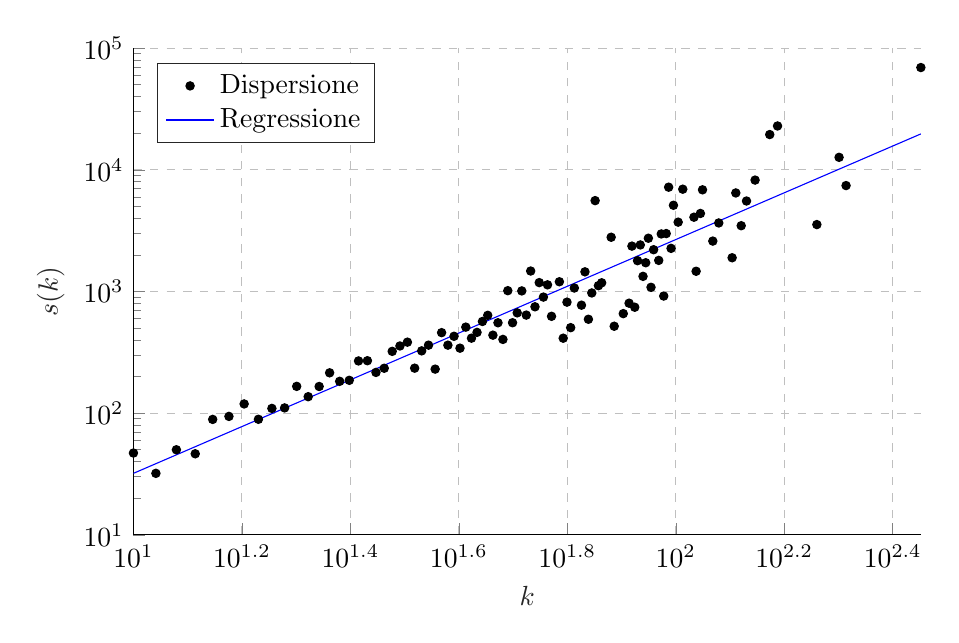
\begin{tikzpicture}
    \definecolor{mycolor1}{rgb}{0.00000,0.44700,0.74100}%
    %
    \pgfmathsetlengthmacro\plotWidth{10cm}
    \pgfmathsetlengthmacro\plotHeight{0.618*\plotWidth}

    % \renewcommand\labelSize{10}
    % \renewcommand\tickSize{9}
    % \renewcommand\legendSize{9}

    \begin{axis}[%
        name=SVsD,
        width=\plotWidth,height=\plotHeight,
        scale only axis,
        % at={(0.758in,0.481in)},
        scale only axis,
        xmin=10,xmax=283,
        ymin=10,ymax=100000,
        xlabel={$k$},ylabel={$s(k)$},
        xlabel style={font=\dimTesto{\labelSize}\color{white!15!black}},
        ylabel style={font=\dimTesto{\labelSize}\color{white!15!black}},
        xticklabel style={font=\dimTesto{\tickSize}},
        yticklabel style={font=\dimTesto{\tickSize}},
        xmode=log,ymode=log,
        xmajorgrids,ymajorgrids,
        xminorticks=true,yminorticks=true,
        axis x line*=bottom,axis y line*=left,
        axis background/.style={fill=white},
        grid style={dashed},
        legend pos=north west,
        legend style={
            font=\dimTesto{\legendSize},
            legend cell align=left,
            align=left,
            draw=white!15!black
        }
    ]
        %\begingroup Dispersione
            \addplot[
                only marks,
                mark=*,
                mark options={},
                mark size=1.5000pt,
                color=black,
                fill=black
            ] table[row sep=crcr] {%
                x	y\\
                10	47\\
                11	32\\
                12	50\\
                13	46.3333333333333\\
                14	88.8\\
                15	94\\
                16	119\\
                17	89\\
                18	109.333333333333\\
                19	110.4\\
                20	166\\
                21	136.5\\
                22	165.6\\
                23	214.5\\
                24	182.6\\
                25	186.111111111111\\
                26	268.5\\
                27	269.692307692308\\
                28	216.1\\
                29	233.833333333333\\
                30	322\\
                31	356.428571428571\\
                32	383.142857142857\\
                33	234.2\\
                34	325\\
                35	362\\
                36	230\\
                37	458.727272727273\\
                38	362\\
                39	428.285714285714\\
                40	342\\
                41	509.3\\
                42	413.2\\
                43	461\\
                44	566.8\\
                45	636.666666666667\\
                46	437.4\\
                47	553\\
                48	403.6\\
                49	1015\\
                50	553.333333333333\\
                51	667.25\\
                52	1010.66666666667\\
                53	639.5\\
                54	1472.5\\
                55	748.333333333333\\
                56	1182.66666666667\\
                57	899\\
                58	1134\\
                59	625\\
                61	1202\\
                62	413\\
                63	817\\
                64	504.25\\
                65	1067.5\\
                67	771.5\\
                68	1450\\
                69	591\\
                70	972.333333333333\\
                71	5581\\
                72	1116\\
                73	1178.66666666667\\
                76	2791\\
                77	518\\
                80	657.5\\
                82	801\\
                83	2359.33333333333\\
                84	742\\
                85	1791\\
                86	2413\\
                87	1331\\
                88	1722.5\\
                89	2739\\
                90	1082\\
                91	2204\\
                93	1801\\
                94	2971\\
                95	917\\
                96	2992.66666666667\\
                97	7198\\
                98	2261.5\\
                99	5111\\
                101	3714\\
                103	6930\\
                108	4078\\
                109	1466\\
                111	4378\\
                112	6849\\
                117	2595\\
                120	3658\\
                127	1893\\
                129	6455\\
                132	3472\\
                135	5541\\
                140	8233\\
                149	19490\\
                154	22926\\
                182	3547\\
                200	12665\\
                206	7422\\
                283	69293\\
            };
            \addlegendentry{Dispersione}
        %\endgroup

        %\begingroup Regressione
            \addplot [color=blue]
            table[row sep=crcr]{%
                10	31.995945118944\\
                11	38.4276028809283\\
                12	45.4218949382162\\
                13	52.9750006283438\\
                14	61.083428931969\\
                15	69.7439676467801\\
                16	78.9536433797812\\
                17	88.7096895015931\\
                18	99.00952008918\\
                19	109.850708458133\\
                20	121.230969270766\\
                21	133.148143470945\\
                22	145.600185482528\\
                23	158.585152241563\\
                24	172.101193729532\\
                25	186.146544746954\\
                26	200.719517720736\\
                27	215.818496379859\\
                28	231.441930165711\\
                29	247.588329268078\\
                30	264.256260197235\\
                31	281.444341818027\\
                32	299.15124178414\\
                33	317.375673320749\\
                34	336.116392311833\\
                35	355.372194655065\\
                36	375.14191385264\\
                37	395.424418810948\\
                38	416.218611825753\\
                39	437.523426732715\\
                40	459.337827205729\\
                41	481.660805187836\\
                42	504.491379441347\\
                43	527.828594205477\\
                44	551.671517951171\\
                45	576.019242224005\\
                46	600.870880567107\\
                47	626.225567516909\\
                48	652.082457665364\\
                49	678.440724782908\\
                50	705.299560997063\\
                51	732.658176022104\\
                52	760.515796435666\\
                53	788.871664998561\\
                54	817.725040014483\\
                55	847.075194726508\\
                56	876.921416747705\\
                57	907.263007523281\\
                58	938.099281822038\\
                59	969.429567255039\\
                61	1033.56954346682\\
                62	1066.37794969122\\
                63	1099.67779714075\\
                64	1133.46847124613\\
                65	1167.74936786812\\
                67	1237.77946225526\\
                68	1273.52750094671\\
                69	1309.76344341059\\
                70	1346.48673292058\\
                71	1383.69682138325\\
                72	1421.39316908376\\
                73	1459.5752444424\\
                76	1577.0306378696\\
                77	1617.15046280896\\
                80	1740.40709870789\\
                82	1824.98769939715\\
                83	1867.99944921639\\
                84	1911.49155591622\\
                85	1955.46356980763\\
                86	1999.91504693729\\
                87	2044.8455489482\\
                88	2090.25464294529\\
                89	2136.14190136572\\
                90	2182.50690185373\\
                91	2229.34922713976\\
                93	2324.46420776204\\
                94	2372.73605295883\\
                95	2421.48360246015\\
                96	2470.70646275207\\
                97	2520.40424476192\\
                98	2570.57656376264\\
                99	2621.22303928018\\
                101	2723.9369586992\\
                103	2828.54304094681\\
                108	3098.31757834956\\
                109	3153.68556787623\\
                111	3265.83189579789\\
                112	3322.60956603761\\
                117	3613.52990409436\\
                120	3793.69623035894\\
                127	4230.40511850972\\
                129	4359.36521991717\\
                132	4556.28523080551\\
                135	4757.37441684874\\
                140	5101.768087655\\
                149	5750.70581991192\\
                154	6127.298860346\\
                182	8446.88808673975\\
                200	10125.3695327078\\
                206	10717.2022330741\\
                283	19730.3233094093\\
            };
            \addlegendentry{Regressione}
        %\endgroup
    \end{axis}

    \redefineTikZbounds{SVsD}{SVsD}
\end{tikzpicture}%%
            }%
            \caption{Forza in funzione del grado per la Sardegna.}%
            \label{figStrenghtVsDegree20}%
        \end{figure}%
